%%%%%%%%%%%%%%%%%%%%%%%%%%%%%%%%%%%%%%%%%%%%%%%%%%%%%%%%%%%%%%%%%%%%%%%%%%%%%%%
%optimization.tex: Detector Optimization
%%%%%%%%%%%%%%%%%%%%%%%%%%%%%%%%%%%%%%%%%%%%%%%%%%%%%%%%%%%%%%%%%%%%%%%%%%%%%%%%
\chapter{Detector Design and Optimization}
\label{sec:optimization_chapter}
%%%%%%%%%%%%%%%%%%%%%%%%%%%%%%%%%%%%%%%%%%%%%%%%%%%%%%%%%%%%%%%%%%%%%%%%%%%%%%%%

\ac{EBEX} employed a kilopixel array of \ac{TES} bolometers, described in Section~\ref{sec:tes_bolometer}. 
These types of detectors were used on ground-based telescopes, like the Atacama Pathfinder Experiment and the South Pole Telescope. 
We modified the design, described in Section~\ref{sec:detector_design}, in order to optimize the detectors to take advantage of the space-like environment in which \ac{EBEX} was flown.

%\textcolor{red}{Is it necessary/helpful to point to the sections here?}

%%%%%%%%%%%%%%%%%%%%%%%%%%%%%%%%%%%%%%%%%%%%%%%%%%%%%%%%%%%%%%%%%%%%%%%%%%%%%%%%
% TES Bolometer Theory {{{
%%%%%%%%%%%%%%%%%%%%%%%%%%%%%%%%%%%%%%%%%%%%%%%%%%%%%%%%%%%%%%%%%%%%%%%%%%%%%%%%
\section{Bolometer Theory}
\label{sec:tes_bolometer}
%%%%%%%%%%%%%%%%%%%%%%%%%%%%%%%%%%%%%%%%%%%%%%%%%%%%%%%%%%%%%%%%%%%%%%%%%%%%%%%%

%\textcolor{red}{Acronyms is failing us ... the figure descriptions are the first place they appear ... how do we fix this??? FIXED... BUT DON'T REMEMBER HOW :/}

%\textcolor{red}{Describe how a bolometer works. Power to temperature detector.}
% Need: cartoon. }


A bolometer is an absorber with some heat capacity weakly thermally coupled to a bath, Figure ~\ref{fig:bolometer_cartoon}. 
%Bolometers absorb power and measure the resultant change in temperature. 
The heat capacitive element absorbs radiation and the resultant change in temperature is measured with a thermistor.  
A \ac{TES} bolometer has a superconductor as its thermistor. 
A superconductor is a special material which has a normal resistance until it drops below its critical temperature, at which point its resistance drops to zero, Figure~\ref{fig:r_vs_t}. 
The \ac{TES} is called such because it is a sensor operated on the edge of its superconducting transition, where there is a steep change in resistance as a function of temperature. 
\textcolor{red}{(Do you have time to add a thermometer or something to the chunk of heat capacity to show that's what you're measuring the temperature of?)}

\begin{figure}[htp]
\begin{center}
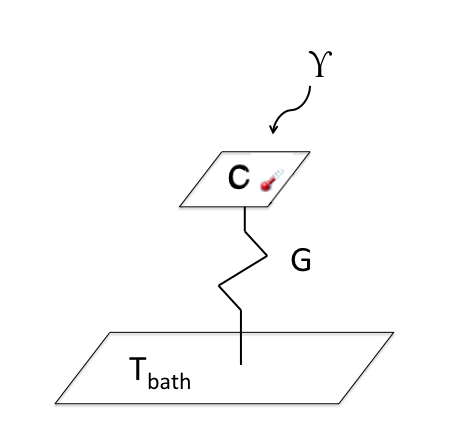
\includegraphics[height=2.5in]{figures/bolometer_cartoon}
\caption{Cartoon bolometer with incoming radiation, $\gamma$. There is an absorber, with heat capacity C, weakly coupled, with thermal conductance G, to a reservoir at $T_{bath}$. A thermistor measures the change in temperature due to the power absorbed. \label{fig:bolometer_cartoon} }
\end{center}
\end{figure}

\begin{figure}[htp]
\begin{center}
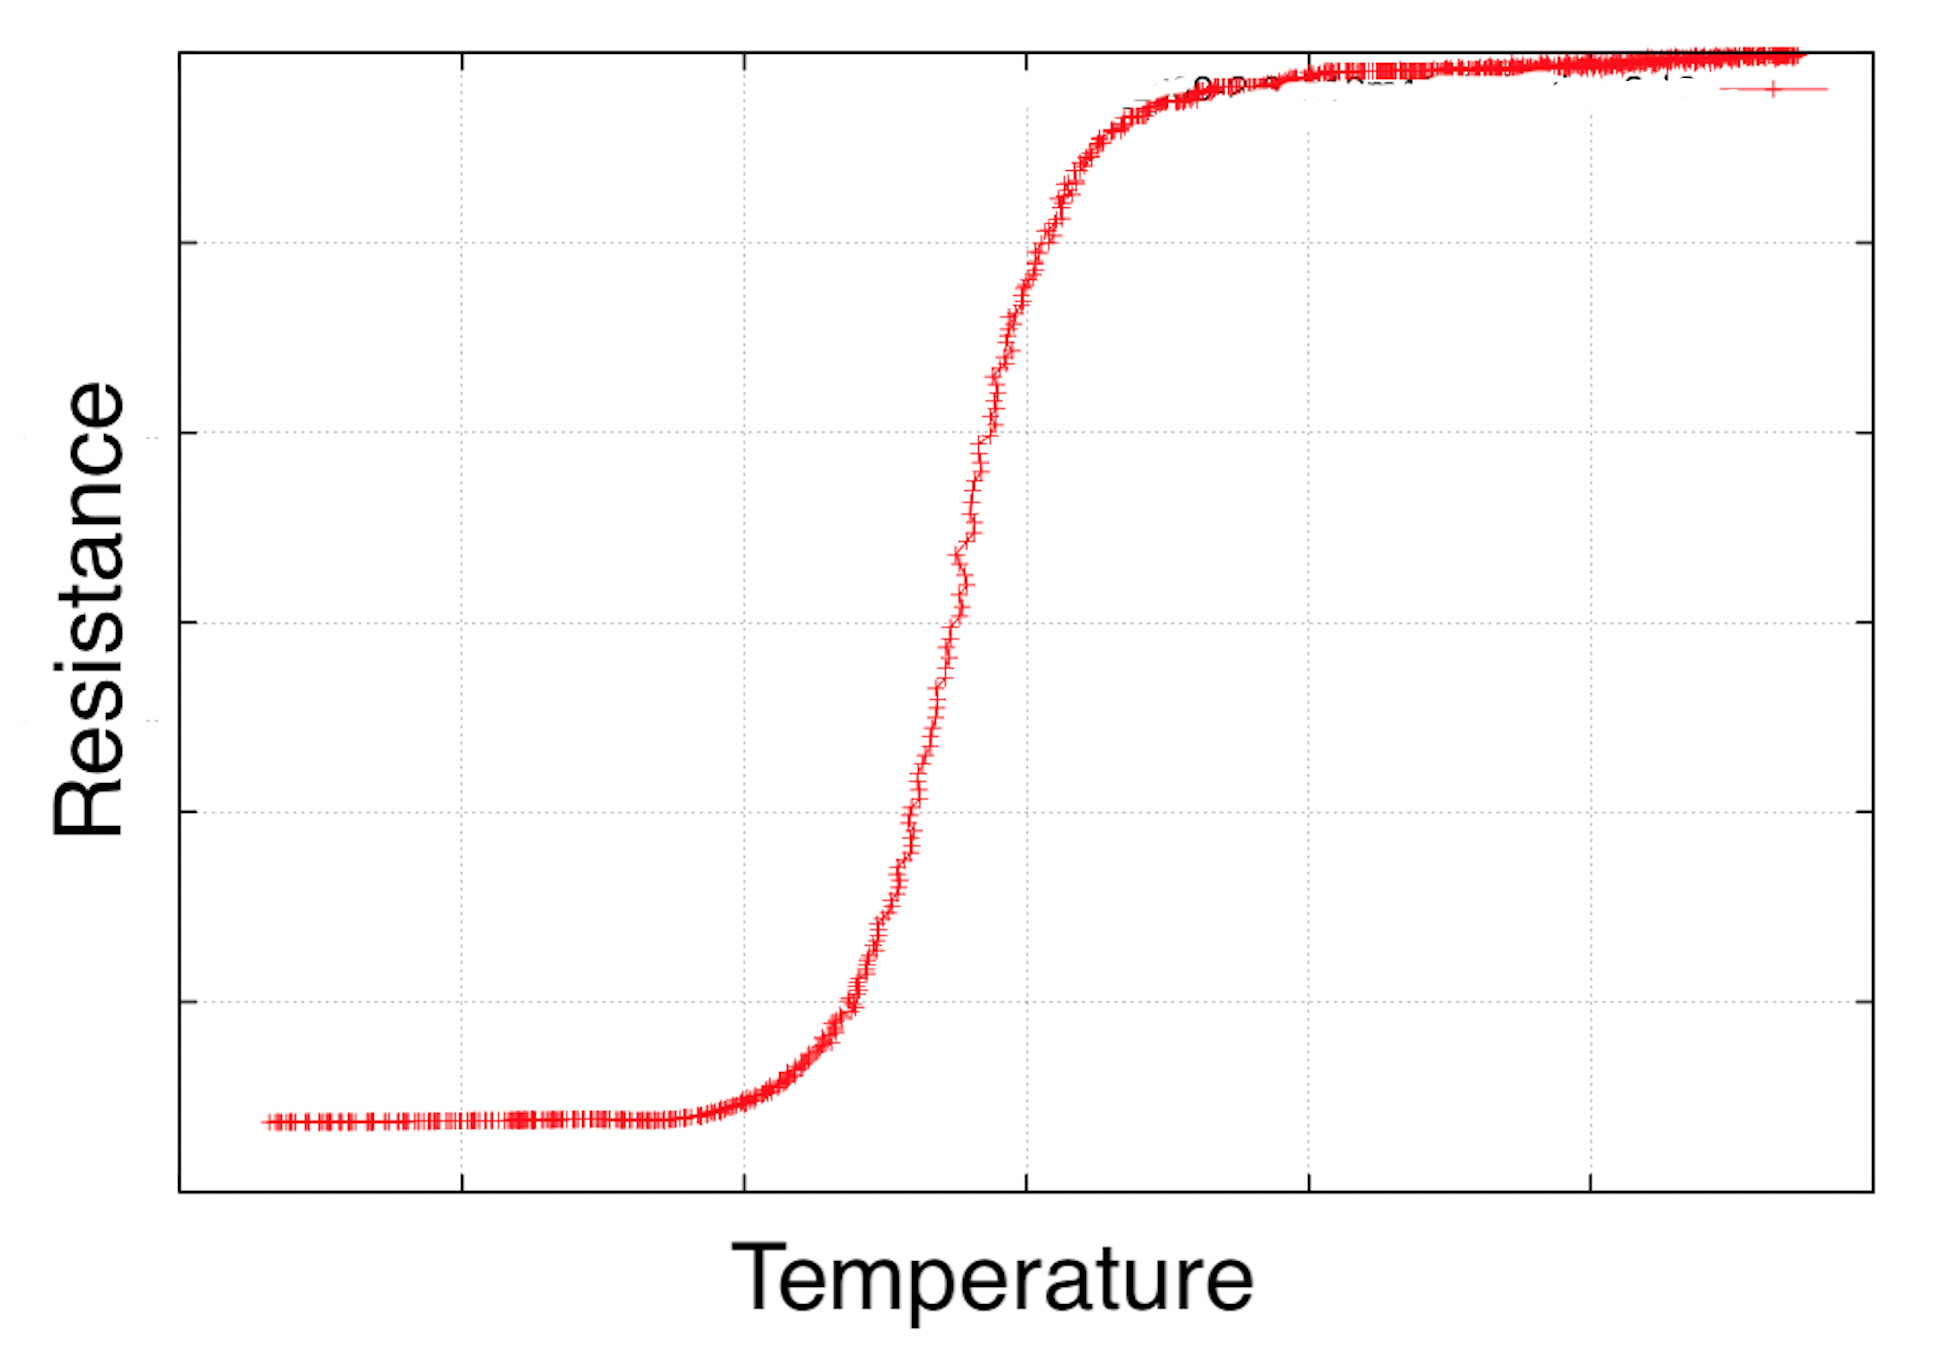
\includegraphics[height=2.5in]{figures/RvsT_for_thesis.png}
\caption{Resistance versus temperature for an \ac{EBEX} \ac{TES} bolometer. As the temperature goes from high to low, the \ac{TES} goes from normal (finite resistance) to superconducting (zero resistance). The region in between is the transition and this is where the \ac{TES} is biased for operation. 
%\textcolor{red}{Make this figure prettier. Need to be able to read axes and their labels OR \textit{remove them}. Say where metal is normal and where it's superconducting and where it's transitioning and where the detector is operated.} 
\label{fig:r_vs_t} }
\end{center}
\end{figure}

%\textcolor{red}{Describe negative electrothermal feedback.}

%\textcolor{red}{For a moment here, just put down some words describing how it works. You can and will return to make it more technical and correct.}
To operate the detector, a voltage bias is applied across the \ac{TES}. 
The voltage bias provides Joule heating of $\frac{V^{2}_{bias}}{R}$.
The voltage bias is chosen such that the detector is heated just enough to hold the \ac{TES} between normal and superconducting. 
In steady-state, there is a constant power flow from the detector to the bath. 
Negative electrothermal feedback holds the detector at the edge of its transition. 
When the radiative load changes, the \ac{TES} warms (cools). 
This change in temperature moves the detector up (down) its R vs T curve. 
%That is, the resistance of the \ac{TES} increases (decreases) in response to an increase (decrease) in radiative load. 
In response to the increase (decrease) in resistance, the Joule heating decreases (increases) and the detector cools (warms). 
For small changes in temperature, this feedback holds the detector on the edge of the transition. 
The voltage bias is constant and so the excursions in resistance change the current through the detector and this is what we measure. 
For flight, we calibrate on a known source in the sky to determine how much the current measured changes given a known amount of power from the sky.   

\textcolor{red}{You need to include the math to describe negative electrothermal feedback more accurately. And then reference that stuff!}

\textcolor{red}{What are the other essential pieces to explaining how a bolometer works?}

\textcolor{red}{Does it make sense to talk about the four sources first and then provide the expression for total NEP? Or to first provide the expression and then derive/talk about each source?}

\textcolor{red}{Figure out how to properly add Mather 1982 applied optics bolometer noise paper to bibfile and reference. Also add Lamarre, "Photon noise in photometric instruments at far-infrared and submillimeter wavelengths", applied optics, vol 25, no 6, 15 march 1986 (he's not there)}


The sensitivity of the instrument is quantified by the \ac{NEP}. 
\ac{NEP} is defined as the absorbed power required to produce a signal-to-noise ratio of one in an electrical bandwidth of one~Hz. 
Though \ac{NEP} is a measure of signal-to-noise, we will use the terms noise and \ac{NEP} interchangeably. 
\textcolor{red}{That sounds like a stupid idea.}
There are four main contributors to the \ac{TES} bolometer \ac{NEP}: electronic/readout noise, Johnson noise, phonon noise, and photon noise. 
%not important?
%Note, sometimes \ac{NEP} is instead defined as the \textit{incident} power required to produce a signal-to-noise ratio of one in an electrical bandwidth of one~Hz, \textcolor{red}{cite who??}.
The total predicted detector \ac{NEP}, $N$, is given by 
\begin{equation}
N^{2} = N_{photon}^2 + N_{phonon}^2 + \frac{1}{S_I^2} ( N_{Johnson}^2 + N_{readout}^2 )
\end{equation}
\begin{equation}
= 2h\nu P_{rad} + \xi \frac{P_{rad}^2}{\Delta \nu} + \gamma 4k_{B} T^2 G + \frac{1}{S_I^2} (\frac{4k_BT}{R} + N_{readout}^2 )
\label{eq:nep}
\end{equation}
where $h$ is Planck's constant, $\nu$ is the center of the observation frequency band, $P_{rad}$ is the radiative power absorbed by the bolometer, $\xi$ is a unitless number between zero and one quantifying the contribution of photon correlation noise, $\Delta \nu$ is the width of the observation frequency band, $\gamma$ is a unitless number between zero and one accounting for the temperature gradient along the link from the \ac{TES} to the bath, $k_{B}$ is Boltzmann's constant, $T$ is the \ac{TES} temperature, $G$ is the bolometer dynamic thermal conductance, $S_{I}$ is the bolometer current responsivity, and $R$ is the \ac{TES} resistance \citep{Mather1982a}. 

The electronic and readout noise is noise due to XXX. 

The Johnson noise is due to XXX (the \ac{TES} being a resistor at a finite temperature). 

The phonon noise is due to the motion of the thermal carriers, phonons, along the weak thermal link. 
If the motion were ballistic versus another kind of transport, then XXX. 

The photon noise is due to the particle nature of photons and the Poisson statistics which govern their arrival. 
This is often referred to as shot noise.
Bolometers have been designed and understood such that the the fundamental limit of the \ac{NEP} is set by the photon arrival statistics. 
There is another source of noise from the photons if their arrivals are correlated, that is if the photons tend to arrive in bunches. 
This is called photon correlation or bunching noise. 
The degree to which this noise source contributes to the bolometer \ac{NEP} is not agreed upon, \cite{Richards}. 
%\textcolor{red}{who says this? richards. and he says van vliet and mather do one thing and pike and lamarre do other things. can I just reference richards? or do I have to refer to all these other folks?}
This disagreement is encapsulated in the factor of $\xi$ which is multiplied by the noise one would have in the case of complete correlation.
$\xi$ can take on a value between zero (no correlation) and one (completely correlated).
There is no correlation when the "beam is produced by an incoherent source and is uniformly distributed over the beam throughput, which is large with respect to the entendue of coherence $\nu^{2}/c{2}$" \cite{Lamarre}.
There is complete correlation in the case of telescopes "observing sources with angular diameters much smaller than the diffraction pattern" \cite{Lamarre}. 
\ac{EBEX} is a telescope observing the \ac{CMB}, which is a uniform source across the sky which occupies a large number of entendues of coherence. 
So, Lamarre would argue, $\xi$ should be zero?
But. We have a diffraction limited beam where our throughput is exactly $A\Omega = \lambda^{2}$.
\textcolor{red}{What is the argument for keeping this second photon noise term??}


%%%%%%%%%%%%%%%%%%%%%%%%%%%%%%%%%%%%%%%%%%%%%%%%%%%%%%%%%%%%%%%%%%%%%%%%%%%%%}}}



%%%%%%%%%%%%%%%%%%%%%%%%%%%%%%%%%%%%%%%%%%%%%%%%%%%%%%%%%%%%%%%%%%%%%%%%%%%%%%%%
% Detector Design Modifications for Space-Like Environment {{{
%%%%%%%%%%%%%%%%%%%%%%%%%%%%%%%%%%%%%%%%%%%%%%%%%%%%%%%%%%%%%%%%%%%%%%%%%%%%%%%%
\section{Detector Design}
\label{sec:detector_design}
%%%%%%%%%%%%%%%%%%%%%%%%%%%%%%%%%%%%%%%%%%%%%%%%%%%%%%%%%%%%%%%%%%%%%%%%%%%%%%%%

The \ac{EBEX} bolometers were fabricated on a silicon device wafer, the thickness of which depended on the observation frequency band, glued to a thick silicon backing wafer.
The left panel of Figure~\ref{fig:bolo_and_bling} is a photograph of a single \ac{EBEX} bolometer. 
The absorber, to which radiation coupled, was a spider web silicon nitride web. 
A silicon etch carved away the silicon underneath so that the web was actually suspended in space.
The link to the bath was provided by eight legs which attached the web to the silicon wafer. 
The heat capacity was provided by a gold waffle, called bling, in the center. 
The \ac{TES} itself was an AlTi bilayer in the shape of a 19 x 19~$\mu m^{2}$ square located at the bottom of the bling, overlapping the bling on the left edge, right panel of Figure~\ref{fig:bolo_and_bling}.

\begin{figure}[ht!]
\begin{center}
%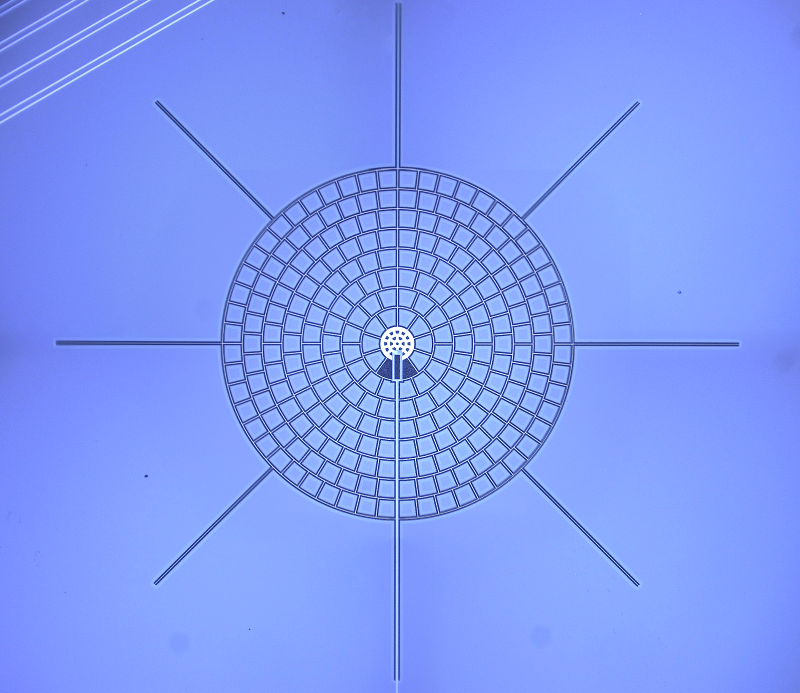
\includegraphics[width=0.49\columnwidth]{figures/bolometer_photo.png}
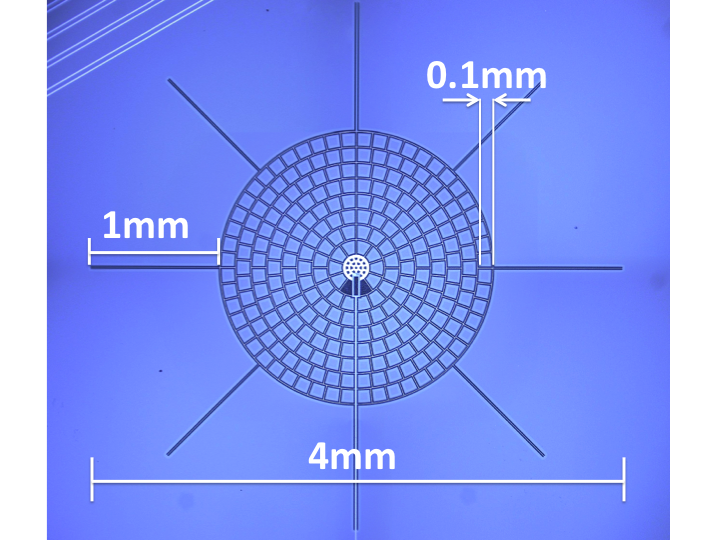
\includegraphics[width=0.49\columnwidth]{figures/fullpixel1_v4_small_annotated.png}
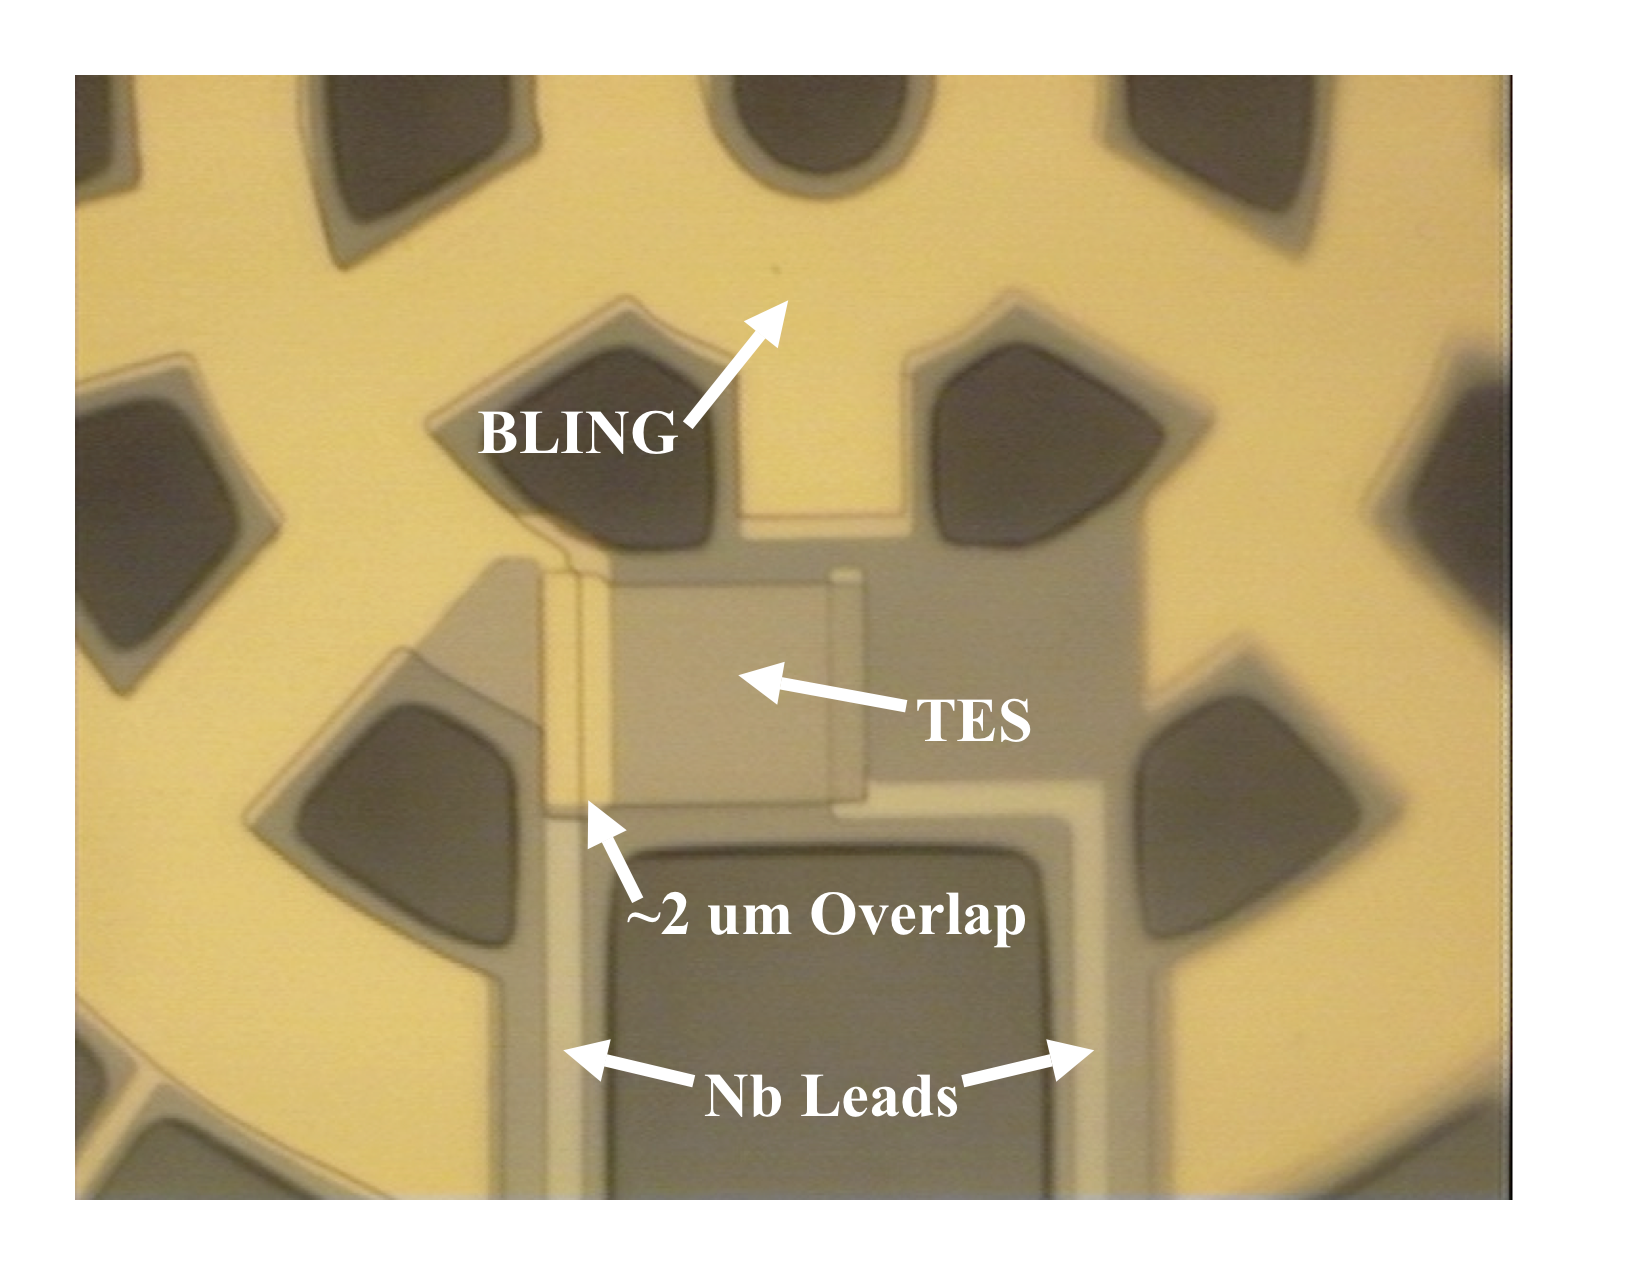
\includegraphics[width=0.45\columnwidth]{figures/EBEX_BLINGTES_Annotated.png}
\caption{Left: One \ac{EBEX} 150~GHz spiderweb \ac{TES} bolometer. The light blue is the silicon wafer on which the detectors were fabricated. The dark blue is open space where the silicon was etched away. Running above the center of the etched out area are the thin silicon nitride strings of the spider web. The spider web is attached to the wafer at the end of each of the spokes. The gold waffle bling in the center provides the heat capacity. Right: A zoom of the bling and the \ac{TES}. The \ac{TES} is a square near the bottom of the bling and is coupled to the bling via the overlap on its left side. The signal travels out the niobium leads to bond pads at the wafer's edge. Both figures courtesy of Benjamin Westbrook. 
\label{fig:bolo_and_bling} }
\end{center}
\end{figure}

\textcolor{red}{How do I properly say this is Ben's not mine?? Looks like others don't really mention where the figures they didn't make are from ... Hmmm.}

\textcolor{red}{Why do you want to say this anyhow? In the first generation wafers, the bling was a simple circle, but in later designs, the bling was a waffle because it coupled better the absorbed power to the \ac{TES}.}


%Discuss target detector parameters. Be very clear about which changes were made to fabrication process in order to optimize the detector sensitivity for a space-like environment and for EBEX.

1. Ideal normal resistance.  
The target normal resistance for all bands was 1.5~$\Omega$ in order to ensure the detector, when biased in the transition, remained in the stable regime where the detector electrical bandwidth, determined in part by the resistance, exceeded the \ac{TES} thermal bandwidth by at least XXX (CITE PAPER). 
%THIS HAS NOTHING TO DO WITH A SPACE-LIKE ENVIRONMENT, but it does have to do with optimization of multiplexing! and so it's relevant. 

2. Ideal transition temperature for our bath temperature. 

%\textcolor{red}{Need to generate: plot of phonon noise as a function of critical temperature, given a fixed ebex bath temperature of 260~mK.}

\textcolor{red}{For a thermal conductance that follows a power law, what kind of material is n=1 and what about n=3? i.e. why are there our bounds??}

\textcolor{red}{I would like for you to explain why modulating the thickness of the aluminum layer changes $T_{c}$. (see p32 of irwin/hilton paper)}


The \ac{TES} was a bilayer of titanium atop aluminum. 
The titanium thickness was fixed at $\sim$110~nm. 
Depending on the wafer, the aluminum thickness varied from $\sim$30 to 50~nm. 
The critical temperature was controlled by the aluminum layer thickness, where the thinner aluminum layer provided a lower critical temperature (and also a higher normal resistance). 

The phonon noise as a function of the critical temperature $T_{c}$, the power of thermal conductivity $n$,  the power to hold the detector in the transition $P_{sat}$, and the bath temperature $T_{bath}$ is
\begin{equation}
\label{eq:phonon_nep}
\begin{split}
NEP_{phonon}^2 & = \gamma4k_{B}T_{c}G_{dyn} \\
& = 4k_{B}T_{bath}P_{sat}\frac{(n+1)^{2}}{(2n+3)^2}\frac{\left(\frac{T_{c}}{T_{bath}}\right)^{2n+3}-1}{\left( \left(\frac{T_{c}}{T_{bath}}\right)^{n+1}-1\right)^{2}}
\end{split}
\end{equation}
If we assumed $T_{bath}$ was 0.26~K, $P_{sat}$ was 6~pW, and $n$ was in between one and three, then the phonon \ac{NEP} was minimized at a ratio of transition temperature to bath temperature, $\frac{T_{c}}{T_{bath}}$, of $\sim$1.7, Figure~\ref{fig:phonon_nep_vs_temps}. 
The \ac{EBEX} bath temperature was 260~mK and so the target critical temperature for all \ac{EBEX} observation frequency bands was 440~mK.

\begin{figure}[htp]
\begin{center}
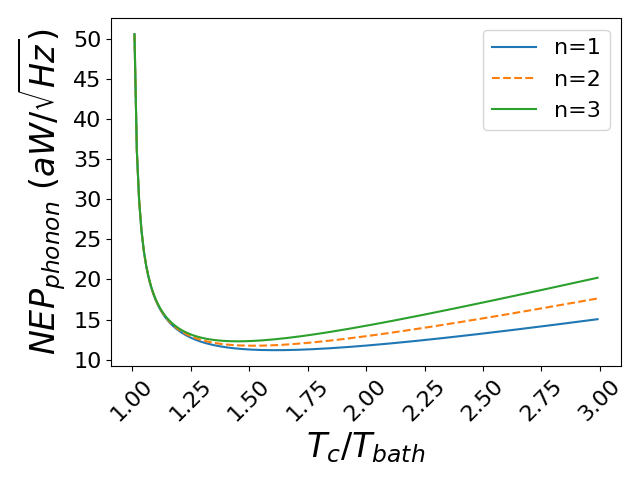
\includegraphics[height=2.5in]{figures/phonon_nep_vs_temperature.png}
\caption{Phonon \ac{NEP} as a function of the ratio of critical temperature to bath temperature for three different values of the thermal conductivity power. The goal was to choose $T_{c}$ such that phonon noise was minimized.
\label{fig:phonon_nep_vs_temps} }
\end{center}
\end{figure}

3. Ideal thermal conductance and heat capacity of TES/web 

\textcolor{red}{It's not obvious that/why a decrease in radiative load can equate to an increase in detector sensitivity. This needs to be spelled out clearly somewhere. Here?}

\textcolor{red}{You're talking about radiative loads and thermal conductance and assuming rather than making the connection between them.}

\textcolor{red}{Add Ben's thesis to bibliography. Is that an acceptable place to reference for the APEX measured load?? If not, which published paper is?}

Ground-based telescopes design their detectors to accommodate the radiative load and fluctuations from the atmosphere. 
Long-duration balloon flights typically float at an altitude of $\sim$120,000~ft, above $\sim$98\% of the atmosphere. 
%\textcolor{red}{Fact check that. - checked csbf website altitude profiles}
For \ac{EBEX} at float, the predicted radiative loads on the detectors were 2.4, 7.3, and 12~pW for the 150, 250, and 410~GHz observation bands. 
%not mentioning 410 here because it's not accessible from the ground and one number is sufficient for comparison purporses
The \ac{EBEX} detectors inherited their initial design from ground-based telescopes, \ac{APEX} and the South Pole Telescope. 
At 150~GHz, the expected radiative load was a factor of roughly 6 less than the $\sim$15~pW load observed by \ac{APEX} \cite{westbrook_thesis}. 
In order to take advantage of the decrease in radiative load at float and increase the detector sensitivity, the fabrication goal was to lower the average thermal conductance from the bolometer to the bath by a factor of 4 to 30~$pW/K$. 
The design goal provided a safety factor of 2.5 in case of unanticipated radiative load or fluctuations.

In order to work towards (achieve?) this goal for the 150~GHz detectors, the spiderweb legs were roughly doubled in length, from 0.5~mm to 1.05~mm, and two of them were decreased in width from 17~$\mu m$ to 6~$\mu m$, right panel of Figure~\ref{fig:bolo_and_bling}. 



4. Ideal time constant

\textcolor{red}{You should talk about time constants... BUT. Your analysis was super simple. And what they did for the paper was much better. So... What do you do? Are you able to write anything intelligent (and correct) about time constants in a small amount of time?}

\textcolor{red}{You really ought to talk about what sets the lower limit (readout) and upper limit (scan speed) on the time constant.}

\textcolor{red}{Also, you can't just say it needs to be held approximately constant if you don't know what the time constants for the ground-based telescopes were!}

\textcolor{red}{Why did we have an observation frequency band dependent target tau??}

\textcolor{red}{I think the following paragraph is not true to how the ideal $\tau$ was decided. Also, isn't $\tau$ also a function of loopgain? (see irwin/hilton p12 on)}
So long as the thermal conductance between the \ac{TES} and the bath was the dominant effect, the time constant of the bolometer was $\tau = C/G$. 
The time constant needed to be held approximately constant at $\sim$20~ms because our telescope was to have roughly the same scan speed as the ground-based telescopes. 
Since the thermal conductance, G, was decreased by a factor of 4 relative to the ground-based detector design, to keep $\tau$ constant, the heat capacity, C, also needed to be decreased by this factor. 
%During the fabrication process for the ground-based detectors, the bling was made of 500-700~nm of gold \textcolor{red}{reference Ben???}. %TOO COMPLICATED. A NICE TO HAVE, NOT A NEED.

The heat capacity was provided by the gold topped silicon nitride bling in the center of the web, see Figure~\ref{fig:bolo_and_bling}. 
For the \ac{EBEX} detectors, we decreased the total thickness of the gold deposited to 20~nm. 

%The dominant heat capacity  dominated by gold deposited  was deposited atop the bling, which was 20~nm of gold atop 1~$\mu m$ of silicon nitride. 





%\emph{FROM EMAIL EXCHANGES WITH BEN.
%We wanted to decrease G, so we roughly doubled the leg length (where you could find space). Do you have pictures of the mask with the original leg length and the final leg length?
%For 150, we pulled out all of the stops we could.  We doubled the length of 7/8 legs from 0.5mm to 1.05 mm. For the 8th leg, we increased it's length by a factor of 3 to 1.45 mm. In addition, we made all the legs expect the one with Nb 6 um wide.  The old design had 2 / 8 with 17 um wide legs. 
%We wanted to decrease Tc, so you messed around with the thickness of the Al layer in our Al/Ti TES sandwich. 
%Specifically we modulate the thickness of the Al (30-50 nm) compared to the Ti layer, which we held at constant thickness (~110nm). More Al means higher Tc and lower Rn (and converse is true).  Technically it's not a sandwhich (that's Shaul's term) it's just a bilayer, Al with Ti on top. Not Al-Ti-Al nor Ti-Al-Ti.
%We wanted to keep the time constant (C/G) the same, so we decreased the heat capacitance by decreasing the thickness of the bling (or we did something else??). 
%So we still had a BLING layer (the waffle pattern at the center of the photos).  However, we didn't add any EXTRA gold here like SPT and APEX had.  The C of the EBEX detectors comes from 20 nm of Gold on a 1um thick layer of Silicon nitride.  Where as the SPT/APEX had the 20nm of gold for the web, the 1 um of Silicon Nitrides, + ~500-700 nm of extra BLING only gold at the center.  Since gold has a large heat capacity, it dominates the total C in the detectors.  I attached a quick memo on this I wrote for Shaul that summarized the changes in heat capacity. 
%Why did we move away from the circle bling design? 
%This is because the waffle pattern has a lower G than the circle so that heat absorbed by the web more efficiently couples to the TES, which ultimately increases optical efficiency (and thus sensitivity) as the TES has time to sense it (i.e it thermalizes) before the heat is dissipated to the bath via the legs.
%Does the CPA track speed control the thickness of the Al in the Al/Ti bilayer?
%Functionally yes.  There are three knobs one could turn: track speed, target power, and argon pressure.  We chose to modulate thickness by varying the track speed while  trying to keep power and pressure constant.
%In the old design, what was the thickness of the other 6 legs?
%The old design had 6, 6 micron wide legs and 2, 17 micron wide legs (one with leads and the one opposite the one with leads). 
%The one with leads also carried the gold heat link.
%> Do you happen to have a schematic that illustrates how we etch the silicon from beneath the silicon nitride? 
%This is my talk from the collab meeting eons ago at McGill.  Pages 7-13 describe the fab process in a cartoon sort of way.  It's the closest thing I have to showing how we release the bolometer structures in presentation form.  If you want the full PPT version let me know.  What basically happens is you etch holes/trenches in the silicon nitride layer and then let the wafer sit in a chamber with XeF2 (Xenon DiFlouride), which etches silicon much much faster than it etches silicon nitride.  The gas finds it's way into the holes and starts digging/etching out the silicon.  After some time a pocket is formed underneath the Silicon nitride (I can make a slide showing this if you need) and the XeF2 starts to isotropically etch (not just down by side to side as well) all of the silicon underneath the structure.  Let me know if you need any more help describing this process. 
%> Did we have the same goal for Tc for each of our wafers?
%> I said it was 1.7 * bath temperature and I think we assumed the bath would be at 270 mK. (giving us a goal of 460 mK)
%> Does this magic number 1.7 change with frequency band?
%Tc = 1.7* Tbath comes from theory for using dieletrics as a thermal bridge.  The plot attached shows that when n = 3, the optimal Tc (the minimum of the dotted lines) is 1.7 * Tbath. However, we used this is a soft criteria and tune our Tc for psat before we did thermal carrier noise.    That means that we basically did have the same target Tc for each wafer, but that was more to tune Psat rather than noise performance.  We did a pretty good job and found that if Tc was around 480-520  we got the Psats we wanted for our 150 and 250/410 GHz wafers (6-8 and 10-12+ pW) for our mask sets. }
%



\begin{table}[ht!]
\centering
%\footnotesize
\begin{tabular}{| c | c c | c c | c c |}\hline
\multicolumn{1}{|c}{Band (GHz)}   &  \multicolumn{2}{|c}{150}   & \multicolumn{2}{|c}{250}   & \multicolumn{2}{|c|}{410}  \\% \hline
                                     & Design & Measured & Design & Measured & Design & Measured  \\ \hline
$R_{n}$ ($\Omega$)            & 1.5  & 1.9  & 1.5  & 1.5  & 1.5  & 1.4  \\
$T_{c}$ (K)                        & 0.44 & 0.45 & 0.44 & 0.49 & 0.44 & 0.47  \\
$\overline{G}$ (pW/K)       & 30   & 39 & 40   & 53 & 50   & 63  \\ \hline
%$\tau_{0}$ (ms)                 & 17 & 88$^\dagger$  & 13  &  46$^\dagger$  &  10 &  57$^\dagger$  \\ \hline
%$C$ (pJ/K)*                         & 0.5  & 3.8$^\dagger$ & 0.5  & 3.3$^\dagger$  & 0.5   & 8.4$^\dagger$  \\ \hline
% Wafer Thickness ($\mu$m)   & \multicolumn{2}{|c|}{150}  & \multicolumn{2}{|c|}{90}  & \multicolumn{2}{|c|}{56}  \\
%$\alpha$ (mm)                &  \multicolumn{2}{|c|}{1.05}   & \multicolumn{2}{|c|}{1.0}   &  \multicolumn{2}{|c|}{0.5}  \\
%$\beta$ (mm)                & \multicolumn{2}{|c|}{1.45} & \multicolumn{2}{|c|}{1.0}  & \multicolumn{2}{|c|}{0.5}  \\ \hline
%\multicolumn{7}{l}{\footnotesize$^\dagger$ Median of measurements on a single wafer at each frequency; see Section~\ref{sec:time_constants}.}\\
%\multicolumn{7}{l}{\footnotesize* Calculated from time constant and thermal conductivity.}
\end{tabular}
\caption{Designed and measured detector parameters for each of the frequency
bands.  The values in the 'measured' columns are median values for 
all detectors on the wafers used for flight.  Description of the measurements and histograms and further discussion 
of the measured values are given in Section~\ref{sec:detector_characterization}.
%For the parameters $\alpha$ and $\beta$, shown in Figure~\ref{fig:Bolometer_Overview} we give the design values. 
%The lithography was generally accurate to within 0.5~$\mu$m.
\label{tab:Design_Params} }
\end{table}


%%%%%%%%%%%%%%%%%%%%%%%%%%%%%%%%%%%%%%%%%%%%%%%%%%%%%%%%%%%%%%%%%%%%%%%%%%%%%}}}